\newif\ifglobal

%%%%%%%%%%%%%%%%%%%%%%%
%%% Compile to view %%%
%%%%%%%%%%%%%%%%%%%%%%%

%%%%%%%%%%%%%%%%%%%%%%%%%%%%%%%%%%%%%%%%%%%%%%%%%%%
%%% Readme:                                     %%%
%%% https://www.overleaf.com/read/bwdjvfjksvjy/ %%%
%%%%%%%%%%%%%%%%%%%%%%%%%%%%%%%%%%%%%%%%%%%%%%%%%%%

% >>> M?: marks a module setting number or important notice

% >>> M4: Set {./relative-path} to external files for this module <<<
\def \modulefiles {./08-BOOTCTRL}
% To add an external file, use:
% (Replace '---' with actual filename)
% '\input{\modulefiles/tables/---.tex}' for tables
% '\includegraphics{\modulefiles/figures/---}' for figures
% '\subfile{\modulefiles/---}' for register files


% >>> M1: This module is in global project? <<<
% 'YES' - uncomment; 'NO' - comment out
\globaltrue

\ifglobal
    \documentclass[main\_\_CN.tex]{subfiles}

\else
    % Font "FandolSong-Regular" used by ctex does not have GSUB table.
    % It causes warnings that do not affect compilation and can be ignored.
    \PassOptionsToPackage{quiet}{fontspec}

    \documentclass[openany, 10pt]{book}

    % >>> M2: In ./00-shared/preamble-trm-module, also find
    %         settings for visibility of todo notes, watermark <<<
    \usepackage{preamble-trm-module}


    % Enable Chinese typesetting
    \usepackage{ctex}

    % >>> M3: Temporary labels in Chinese
    %         you can add your own labels there <<<
    \myexternaldocument{./00-shared/temp-labels-cn}

\fi %\ifglobal


\setcounter{secnumdepth}{4}


% >>> M5: If this module needs any updates in
% './00-shared/preamble-trm-module.sty'
% (include additional package, etc.), contact your module PM
% or create the file './00-shared/changelog.tex' make the
% necessary updates yourself and document them in this file <<<


\begin{document}


% Sets language into which pre-defined bits of text are translated
\selectlanguage{chinese}

% Do not delete this block
\ifglobal
% Add the following front matter if
% this module is outside of global project
\else
    \InputIfFileExists{readme}{}{}
    {\let\clearpage\relax \listoftodos}
    \tableofcontents
    %\listoftables
    %\listoffigures
\fi


%%%%%%%%%%%%%%%%%%%%%%%%%
%%% TRM Module Begins %%%
%%%%%%%%%%%%%%%%%%%%%%%%%

\hypertarget{bootctrl}{}
\chapter{芯片 Boot 控制}
\label{mod:bootctrl}


\section{概述}

Strapping 管脚是指 \chipname{} 芯片的特定管脚，可用于控制 \chipname{} 芯片上电或硬件复位时的一些功能，包括：
\begin{itemize}
    \item 控制 Boot 模式
    \item 控制 ROM 代码日志打印到 UART
\end{itemize}

\chipname{} 共有两个 Strapping 管脚：
\begin{itemize}
    \item GPIO8
    \item GPIO9
\end{itemize}

在芯片复位（请参考 \ref{mod:resclk} \textit{\nameref{mod:resclk}} 章节）过程中，硬件将采样 Strapping 管脚电平存储到锁存器中，并一直保持到芯片掉电。Strapping 管脚锁存的状态可以通过软件从 \hyperref[fielddesc:GPIOSTRAPPING]{GPIO\_STRAPPING} 中读取。



\section{特性}
\begin{itemize}
    \item 共两个 Strapping 管脚：
    \begin{itemize}
        \item GPIO8
        \item GPIO9
    \end{itemize}
    \item 可控制芯片 Boot 模式：
    \begin{itemize}
        \item SPI Boot 模式
        \item Download Boot 模式
    \end{itemize}
    \item 控制 ROM 代码日志是否打印到 UART
    \item Strapping 管脚的锁存值可通过软件从 \hyperref[fielddesc:GPIOSTRAPPING]{GPIO\_STRAPPING} 中读取
\end{itemize}

\section{功能描述}

本小节主要介绍芯片复位时的功能以及控制该功能使用到的 Strapping 组合模式。

\begin{importantlisting}
请使用本章节所介绍的组合，其它组合可能会导致不可控结果。
\end{importantlisting}

\subsection{默认配置}

GPIO9 默认连接内部上拉电阻。如果这一管脚没有外部连接或者连接的外部线路处于高阻抗状态，内部弱上拉将决定这一管脚输入电平的默认值，如表 \ref{tab:bootctrl-default-config-strapping-pins} 所示。

\begin{longtable}[c]{|p{1.5cm}|c|}
\caption{管脚默认上拉/下拉}
\label{tab:bootctrl-default-config-strapping-pins} \\
    \hline
    \rowcolor{lightgray}
  \textbf{管脚} & \textbf{默认值} \\ \hline
  \textbf{GPIO8} & N/A \\ \hline
  \textbf{GPIO9} & 上拉 \\ \hline
\end{longtable}

如需改变 Strapping 管脚的默认值，用户可以应用外部下拉/上拉电阻，或者应用主机 MCU 的 GPIO 来控制 \chipname{} 上电复位时的 Strapping 管脚电平。复位释放后，Strapping 管脚和普通管脚功能相同。

\subsection{Boot 模式控制}\label{sec:boot-mode-control}
复位释放后，GPIO2、GPIO3、GPIO8 和 GPIO9 在复位时的值将共同决定 Boot 模式。表 \ref{tab:bootctrl-boot-mode-control} 列出了 GPIO2、GPIO3、GPIO8 和 GPIO9 的 Strapping 值及其对应的系统启动模式。

\begin{table}[H]
    \centering
\caption{系统启动模式}
\label{tab:bootctrl-boot-mode-control}
\begin{threeparttable}
    \begin{tabular}{ | p{5cm} | c | c | c |c| }
    \hline
    \rowcolor{lightgray}
  \textbf{启动模式} & \textbf{GPIO9} & \textbf{GPIO8} & \textbf{GPIO3} & \textbf{GPIO2}\\ \hline
  SPI Boot 模式 & 1 & x\tnote{1} & x & x \\ \hline
  Joint Download Boot 模式\tnote{2} & 0 & 1 & x & x\\ \hline
  SPI Download Boot 模式\tnote{3} & 0 & 0 & 0 & 1 \\ \hline
  无效组合\tnote{4} & 0 & 0  & x & 0 \\ \hline
\end{tabular}

\begin{tablenotes}
            \item[1] x：任何取值均不会对结果有影响，因此可忽略。
            \item[2] Joint Download Boot 模式：Joint Download Boot 模式下支持以下下载方式：
            \begin{itemize}
                \item UART Download Boot
            \end{itemize}
            \item[3] SPI Download Boot 模式：只有使用 SPI Download Boot 模式时才需要预留 GPIO3 和 GPIO2。 GPIO3 和 GPIO2 默认浮空，在复位时处于高阻抗状态。
            \item[4] 无效组合：该组合会触发意外行为，应当避免。
        \end{tablenotes}
     \end{threeparttable}
\end{table}



在 SPI Boot 模式下，ROM 引导加载程序通过从 SPI flash 中读取程序来启动系统。SPI Boot 模式可进一步细分为以下两种启动方式：
\begin{itemize}
    \item 常规 flash 启动方式：支持安全启动。ROM 引导加载程序将程序从 flash 加载到 SRAM，并执行。在大多数实际应用场景中，上述执行的程序多为二级引导程序，该二级引导程序将启动最终的应用程序。
    \item 直接启动方式：不支持安全启动，程序直接从 flash 中运行。如需使能这一启动方式，请确保下载至 flash 的 bin 文件其前两个字为 0xaedb041d。详细的启动流程，见图 \ref{fig:boot_flow}。
\end{itemize}

在 Joint Download Boot 模式下，用户可通过 UART0 接口将二进制文件下载至 flash，或将二进制文件下载至 SRAM 并从 SRAM 中运行程序。

在 SPI Download Boot 模式下，用户可通过 SPI 接口将二进制文件下载至 flash，或将二进制文件下载至 SRAM 并运行 SRAM 中的程序。


芯片启动的具体流程见图 \ref{fig:boot_flow}。

\begin{figure}[H]
    \centering
    {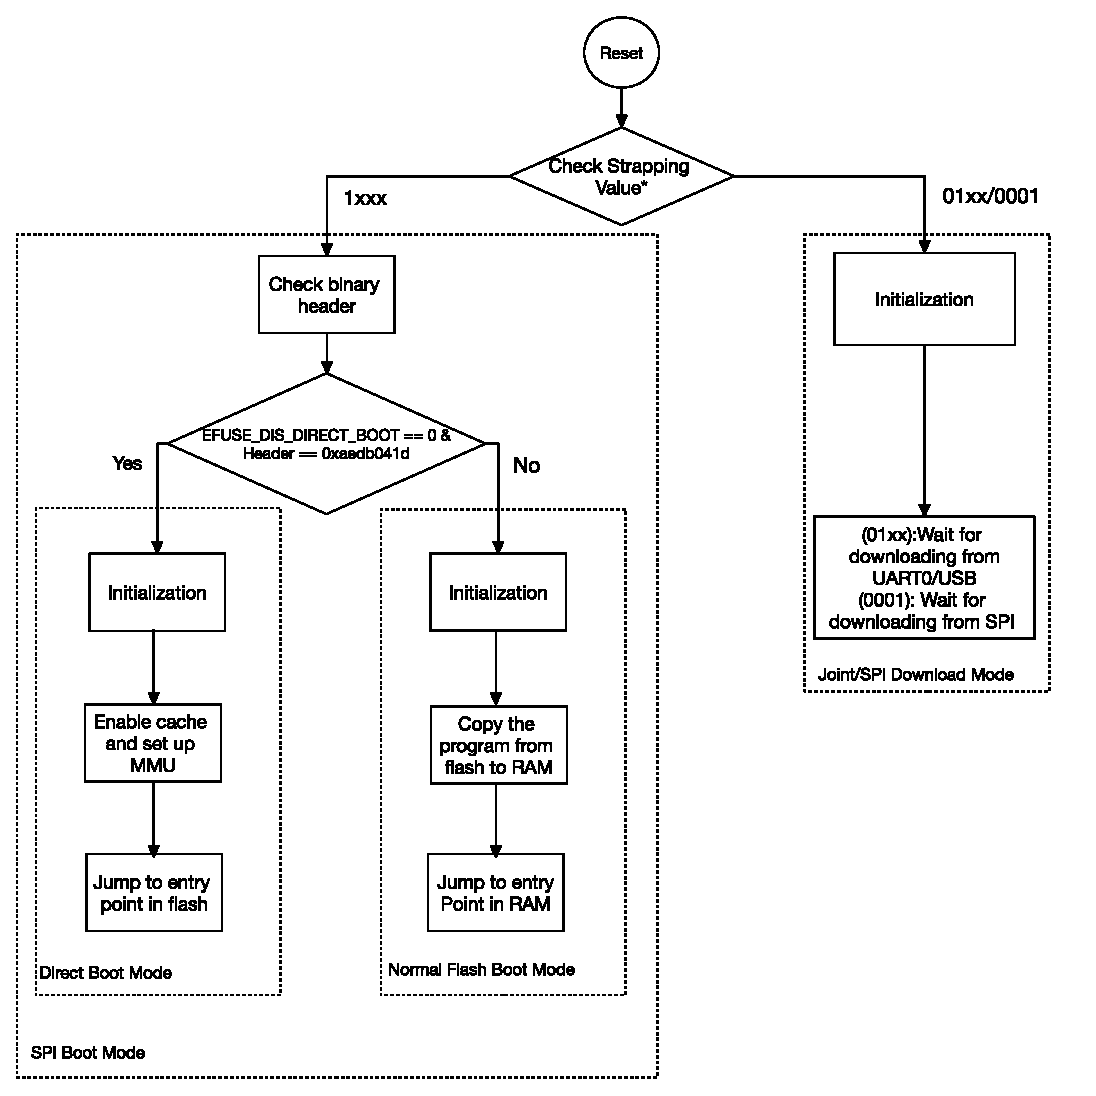
\includegraphics[width=1.0\textwidth]{08-BOOTCTRL/figures/boot_flow_230606.eps}}
    \caption{芯片启动流程}
    \label{fig:boot_flow}
\end{figure}

下面几个寄存器可用于控制启动模式的具体行为：

\begin{itemize}
    \item \hyperref[fielddesc:RTCCNTLFORCEDOWNLOADBOOT]{RTC\_CNTL\_FORCE\_DOWNLOAD\_BOOT}

    软件可通过设置 \hyperref[fielddesc:RTCCNTLFORCEDOWNLOADBOOT]{RTC\_CNTL\_FORCE\_DOWNLOAD\_BOOT}，触发 CPU 复位，将芯片启动模式强制从 SPI Boot 模式切换至 Joint Download Boot 模式。这种情况下，硬件会将 \hyperref[fielddesc:GPIOSTRAPPING]{GPIO\_STRAPPING}[3:2] 的值从 ``1x" 覆盖为 ``01"。

    \item \hyperref[fielddesc:EFUSEDISDOWNLOADMODE]{EFUSE\_DIS\_DOWNLOAD\_MODE}

    如果此 eFuse 设置为 1，则禁用 Joint Download Boot 模式。\hyperref[fielddesc:GPIOSTRAPPING]{GPIO\_STRAPPING} 的值则不受 \hyperref[fielddesc:RTCCNTLFORCEDOWNLOADBOOT]{RTC\_CNTL\_FORCE\_DOWNLOAD\_BOOT} 的影响。
    \item \hyperref[fielddesc:EFUSEENABLESECURITYDOWNLOAD]{EFUSE\_ENABLE\_SECURITY\_DOWNLOAD}

    如果此 eFuse 设置为 1，则在 Joint Download Boot 模式下，只允许读取、写入和擦除明文 flash，不支持 SRAM 或寄存器操作。如已禁用 Joint Download Boot 模式，请忽略此 eFuse。

    \item EFUSE\_DIS\_DIRECT\_BOOT

    如果此 eFuse 设置为 1，则禁用 Direct Boot 模式。

\end{itemize}


\subsection{ROM 代码日志打印控制}

系统在 SPI 启动模式下的早期阶段，GPIO8 与 \hyperref[fielddesc:EFUSEUARTPRINTCONTROL]{EFUSE\_UART\_PRINT\_CONTROL} 一起控制 ROM 代码日志打印。

\begin{table}[H]
    \centering
    \caption{ROM 代码日志打印控制}
    \label{tab:bootctrl-rom-code-printing-control}
    \begin{threeparttable}
    \begin{tabular}{ |p{1.3cm}<{\centering}|p{1.3cm}<{\centering}|p{6.5cm}|}
    \hline
        \rowcolor{lightgray}
    \textbf{eFuse\tnote{1}} &   \textbf{GPIO8}      & \textbf{ROM 代码日志打印} \\\hline
    \multirow{2}*{0} &  \multirow{2}*{x}  & 启动过程中，ROM 代码日志始终打印至 UART，此时 GPIO8 的值被忽略\\\hline
    \multirow{2}*{1}   & 0     & 启动过程中使能打印 \\\cline{2-3}
     & 1       & 启动过程中关闭打印 \\\hline
    \multirow{2}*{2}   & 0     & 启动过程中关闭打印 \\\cline{2-3}
     & 1       & 启动过程中使能打印 \\\hline
     \multirow{2}*{3} &  \multirow{2}*{x}  & 启动过程中始终关闭打印，此时 GPIO8 的值被忽略\\\hline
        \end{tabular}

        \begin{tablenotes}
            \item[1] eFuse: EFUSE\_UART\_PRINT\_CONTROL
        \end{tablenotes}
     \end{threeparttable}
    \end{table}




\end{document}
